% Lecture Template for ME3023 -  Measurements in Mechanical Systems - Tennessee Technological University
% Spring 2020 - Summer 2020 - Fall 2020 - Spring 2021 - Summer 2021
% Tristan Hill, May 07, 2020 - June 12, 2020 - July 08, 2020 - Novemeber 02, 2020 - March 28, 2021 - May 25, 2021
% Module Name: To Err is Human
% Topic 1 - Accuracy and Error

\documentclass[fleqn]{beamer} % for presentation (has nav buttons at bottom)

\usepackage{/home/thill/Documents/lectures/measurements_lectures/measurements_lectures}

\author{ME3023 - Measurements in Mechanical Systems} 

%\newcommand{\MNUM}{2\hspace{2mm}} % Module number
\newcommand{\TNUM}{1\hspace{2mm}} % Topic number 
\newcommand{\moduletitle}{To Err is Human}
\newcommand{\topictitle}{Accuracy and Error} 

\newcommand{\sectiontitleI}{Thought Experiment}
\newcommand{\sectiontitleII}{Accuracy and Error}
\newcommand{\sectiontitleIII}{Estimating Error}
\newcommand{\sectiontitleIV}{Uncertainty Interval}

% custom box
\newsavebox{\mybox}

\title{Lecture Module - \moduletitle}

\date{Mechanical Engineering\vspc Tennessee Technological University}

\begin{document}
	
	\lstset{language=MATLAB,basicstyle=\ttfamily\small,showstringspaces=false}
	
	\frame{\titlepage \center\begin{framed}\Large \textbf{Topic \TNUM - \topictitle}\end{framed} \vspace{5mm}}

% Section 0: Outline
\frame{

\large \textbf{Topic \TNUM - \topictitle} \vspace{3mm}\\

\begin{itemize}

	\item \hyperlink{sectionI}{\sectiontitleI} \vspc % Section I
	\item \hyperlink{sectionII}{\sectiontitleII} \vspc % Section II
	\item \hyperlink{sectionIII}{\sectiontitleIII} \vspc %Section III
	\item \hyperlink{sectionIV}{\sectiontitleIV} \vspc %Section IV

\end{itemize}

}

% Section 1
\section{\sectiontitleI}

\begin{frame}[label=sectionI]
\frametitle{\sectiontitleI}

{\bf Thought Experiment}: Look around the room and choose an object. It can be anything. Ask yourself the following questions. \vspc
\begin{itemize}
\item What is the {\bf\GR true} length of the object? \vspc
\item How can you find the {\bf\GR true} value? Can you measure it? \vspc
\item ...
\end{itemize}

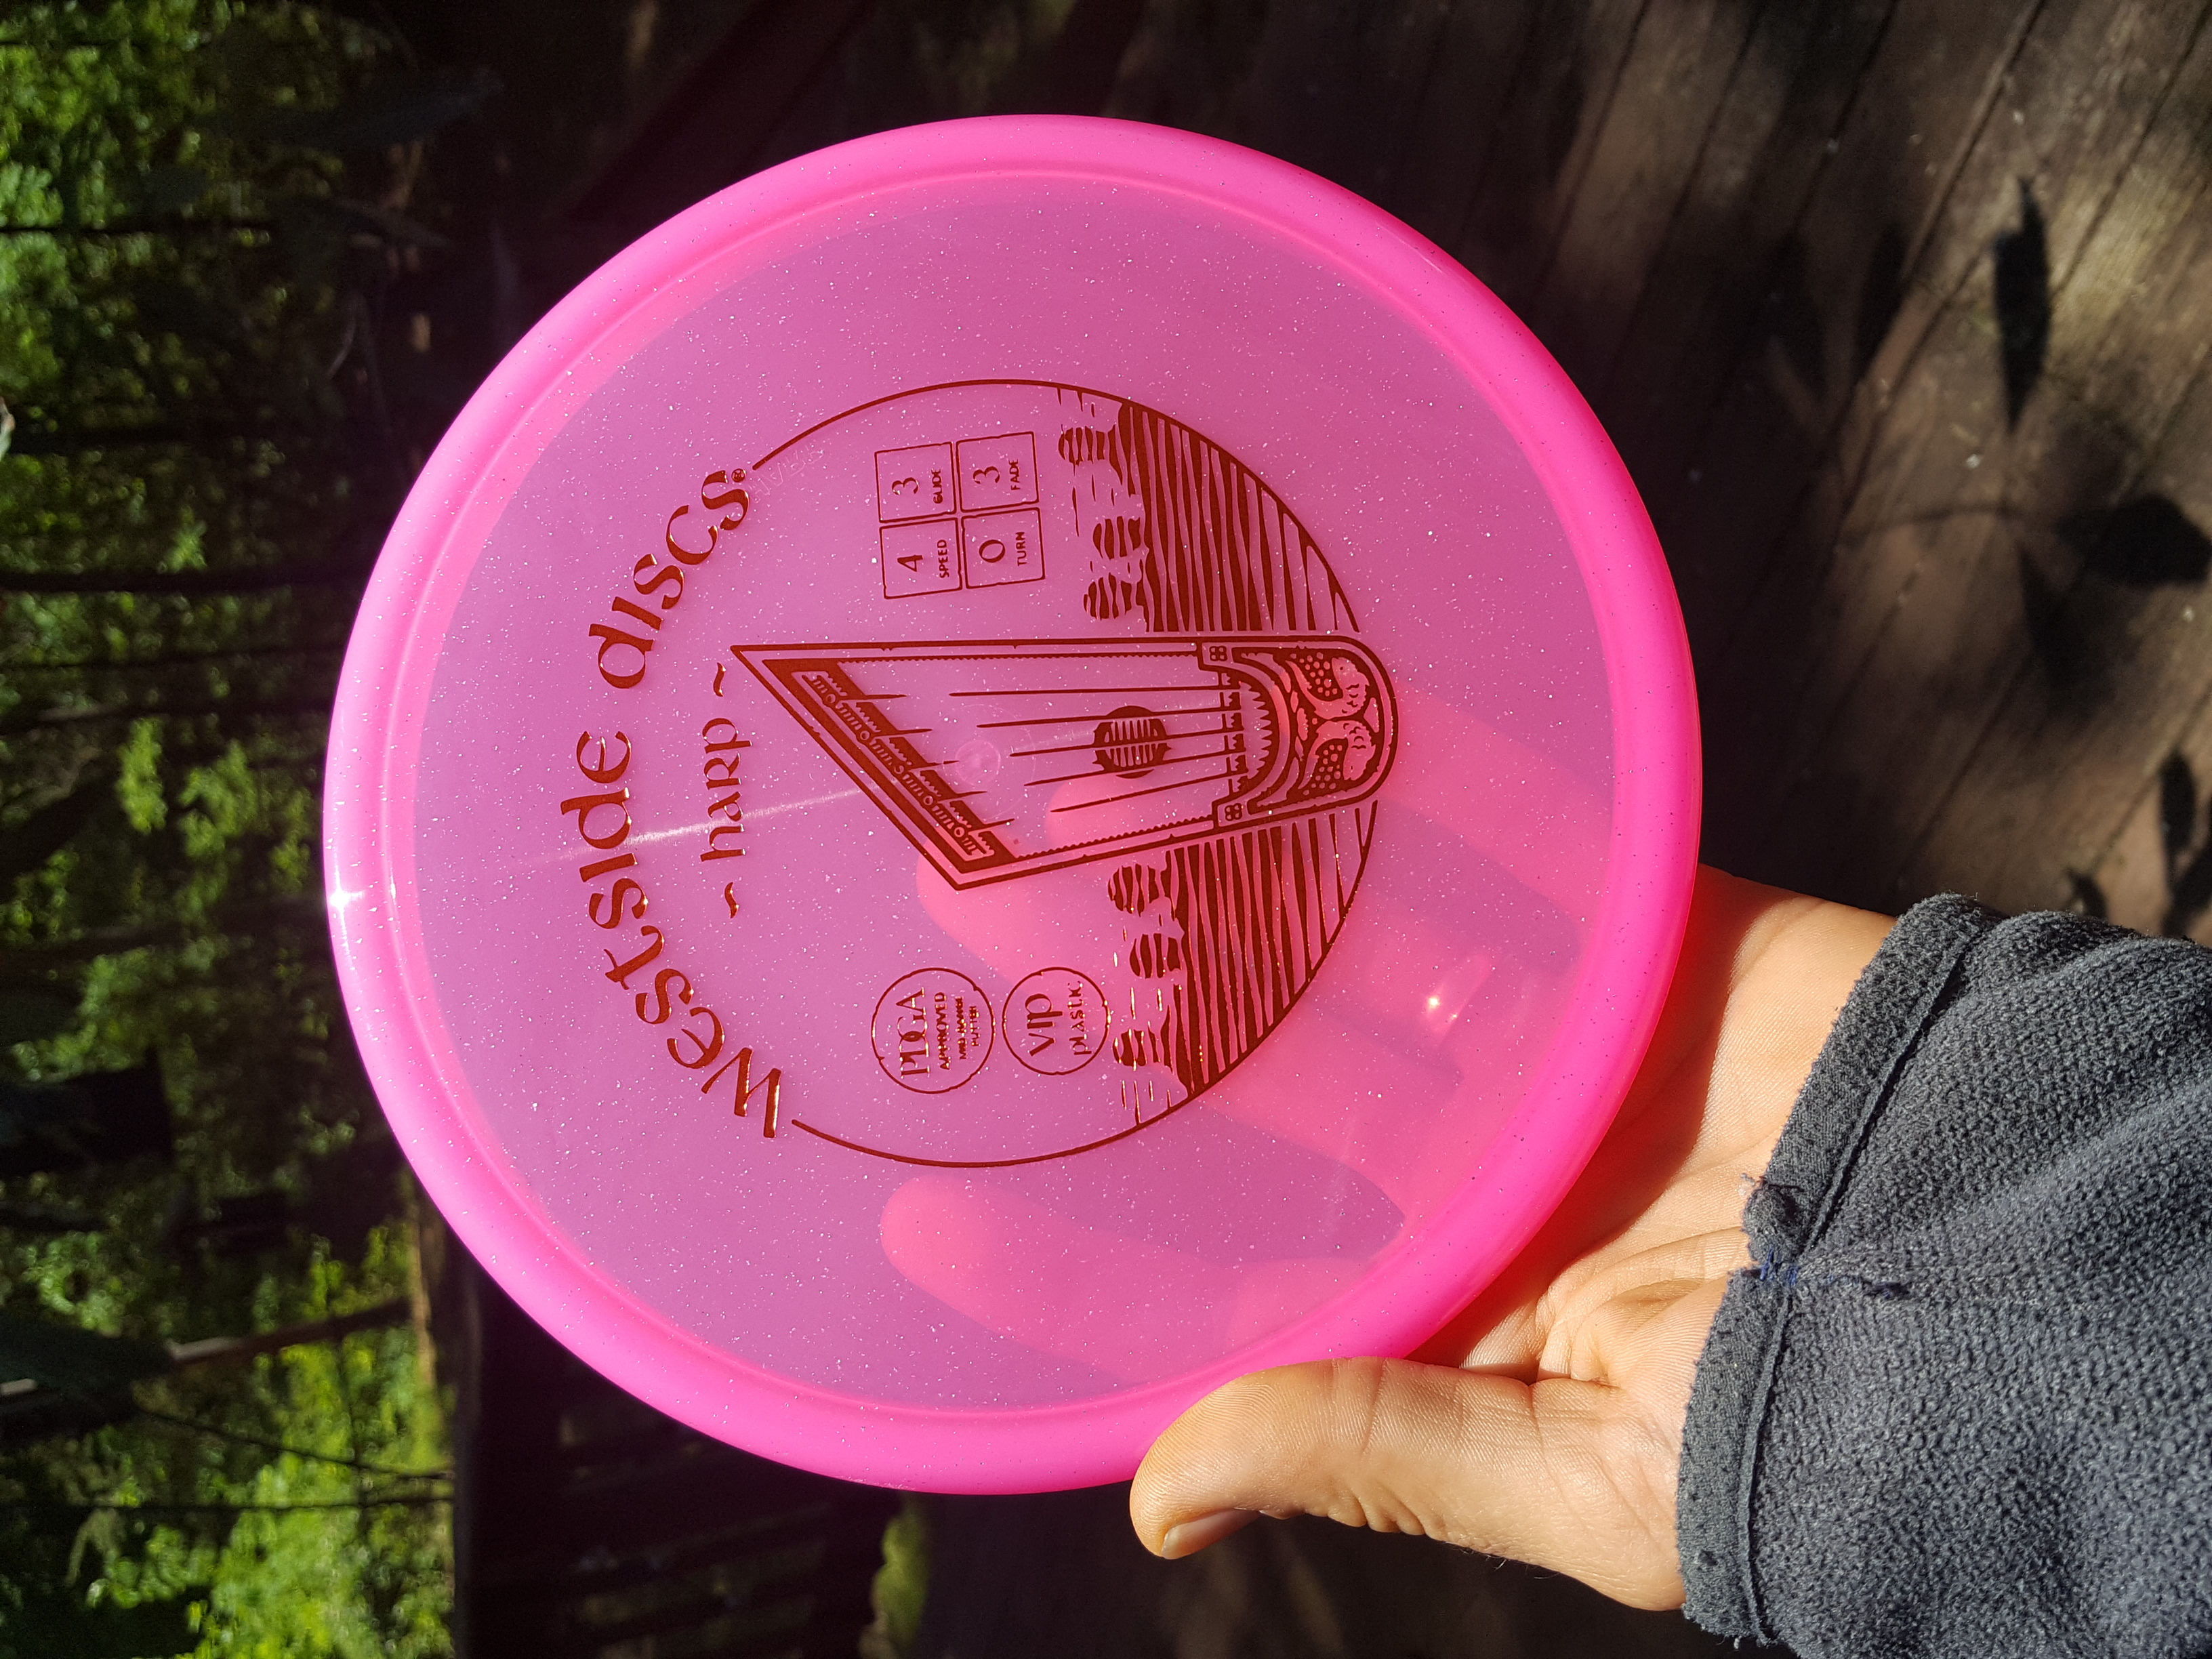
\includegraphics[scale=.025,angle=-90,origin=c]{vip_harp.jpg}
{\tiny Image: T.Hill}
\end{frame}


% Section 2

\begin{frame}[label=sectionII]
\frametitle{\sectiontitleII}


The exact value of a variable is called the \hspcu \hspc \hspcu. The value of the variables as indicated by a
measurement system is called the \hspcu \hspc \hspcu. The \hspcu of a measurement refers to the
closeness of agreement between the measured value and the true value. But the \hspcu \hspc \hspcu is rarely
known \hspcu, and various influences, called \hspcu, have an effect on both of these values. So the
concept of the \hspcu of a measurement is a \hspcu one. \vspcc

\begin{framed}
	%\scalebox{1}{}$\hspace{10mm}{\RD error} = {\BL measured\hspace{1mm}value} - {\GR true\hspace{1mm}value} $}
\end{framed}

\vspace{0mm}
{\tiny Text: Theory and Design of Mech. Meas.}
\end{frame}

% Section 3
\section{\sectiontitleIII}

\begin{frame}[label=sectionIII]
\frametitle{\sectiontitleIII}

The \hspcu \hspc \hspcu can be estimated but cannot be known  \hspcu. In practice a \hspcu value is used in place of the true value. We will discuss this again the the {\it Calibration Module}.


\begin{framed}%\scalebox{1}{$\hspace{20mm} {\PR accuracy} =  \frac{|{\RD error}|}{{\BR reference\hspace{1mm}value}}\times 100 $}
\end{framed}

An estimate of error based using this value is sometimes referred to as \hspcu \hspc \hspcu. \vspc

\end{frame}

% Section 4
\section{\sectiontitleIV}

\begin{frame}[label=sectionIV]
\frametitle{\sectiontitleIV}

``The \hspcu is a numerical estimate of the possible range of the error in a measurement. In any
measurement, the \hspcu is not known exactly since the true value is rarely known exactly. But based on
available information, the operator might feel confident that the error is within certain bounds, a plus
or minus range of the indicated reading. This is the assigned \hspcu.''\vspace{5mm}\\
We will discuss this again the the {\it Uncertainty Module}.\vspace{10mm}\\

{\tiny Text: Theory and Design of Mech. Meas.}
\end{frame}


\end{document}





